\documentclass [11pt]{article}
\usepackage [spanish] {babel}
\usepackage [T1]{fontenc}
\usepackage [utf8]{inputenc}
\usepackage {anysize}
\usepackage {graphicx}
\usepackage [pdfborder = 0 0 0]{hyperref}
\begin{document}
\author{Albert Llop}
\title{\Huge{\textbf{Proyecto de Fin de Carrera} \\ Pizarra Web Compartida}}
\maketitle
\section{Objetivos del proyecto}
Este proyecto surge de la necesidad de realizar presentaciones a distancia, mayoritariamente por videoconferencia. Las videoconferencias están en el día a día de las empresas, y por supuesto, las presentaciones en powerpoint están en la vida diaria de cualquiera. El realizar estas presentaciones a distancia crea una serie de problemas:

\begin{itemize}
	\item Cada \emph{usuario} ve el documento individualmente, por lo cual no hay una sincronía entre lo que todos ven. Cada uno puede estar mirando una hoja distinta, o a un punto distinto.
	\item A diferencia de en una presentación real, el poniente carece de una pizarra o una superficie donde hacer explicaciones cuando las diapositivas no son suficiente.
\end{itemize}

Estas dos carencias básicas hacen que se pierda un gran porcentaje del tiempo de dichas conferencias en \emph{forzar} esa sincronía, con explicaciones constantes de en qué diapositiva se está, o a qué punto mirar, o en simular dicha pizarra, con explicaciones verbales en vez de gráficas. El objetivo básico de este proyecto es, por tanto, buscar una solución a estas carencias en forma de página web, aprovechando para estudiar el mundo de las aplicaciones web interactivas, y profundizando en la comprensión de las capacidades de las tecnologías actuales.

\subsection{Objetivos concretos}

Debido a las limitaciones típicas de los entornos en que muchas empresas tienen sus sistemas (firewalls, falta de plugins en navegadores, etc), el primer objetivo que se establece es el de que sea posible utilizar el servicio desde un navegador web típico, con el mínimo posible de requisitos.

El proyecto en si se puede diferenciar en dos partes, una que sería la \textbf{pizarra} compartida en si, donde se dibujaría, y donde la gente podría ver el documento y los dibujos del ponente; y otra parte diferente que sería el \textbf{sistema} que se encargaría de organizar los distintos documentos y usuarios, es decir, todo el trabajo previo antes de empezar a dibujar (subir el documento, dar permisos para que la gente pueda verlo, etc).

\subsubsection{Sistema}
El sistema debe permitir una serie de acciones:

\begin{description}
	\item[Gestión de Usuario] Se tiene que poder registrar, hacer login y salir. Todas las opciones tienen que ser modificables por el usuario, por ejemplo, la contraseña.
	\item[Gestión de Grupos] Poder crear grupos, invitar a usuarios a dichos grupos.
	\item[Gestión de Pizarras] Cada usuario tiene que poder subir sus documentos y gestionarlos. Tiene que poder invitar a otros usuarios y/o grupos a participar en él.
	\item[Participación en otras Pizarras] Cada usuario tiene que poder ver los documentos a los que ha sido invitado, acceder y salir de ellos.
\end{description}

Se pretende que todo el proceso de registro y manejo sea lo más sencillo posible, tan solo un trámite para lo que realmente importa, que es utilizar la herramienta para ayudar a las presentaciones.

\subsubsection{Pizarra}
Se considera una pizarra como un lugar donde poder escribir, dibujar, al cual se le ha cargado unas imágenes de fondo, que se podrían considerar las diapositivas de una presentación. Una persona que tenga que hacer dos presentaciones a partir de dos archivos distintos, tendrá que crear dos pizarras distintas, e invitar a la gente adecuada. Se puede invitar a gente distinta en cada pizarra que se haya creado. Los objetivos para estas pizarras son los siguientes:

\begin{description}
	\item[Carga de documento] Cada pizarra tiene la posibilidad de añadir un documento que se cargará como imágenes de fondo. La subida de dichas imágenes tiene que ser lo más flexible posible.
	\begin{itemize}
		\item Una por una en formato de imagen JPG/PNG.
		\item Un zip/rar con el conjunto de imágenes.
		\item Mediante un PDF.
		\item (Opcional) Mediante una presentación PowerPoint directamente.
	\end{itemize}
	\item[Multipágina] Cada imagen tiene que ser una página diferente. Se tiene que poder avanzar y retroceder entre ellas.
	\item[Puntero] Se tiene que poder ver el puntero del ``administrador'', de forma que los usuarios pueden ver qué está señalando en ese momento, en vez de esperar a que dibuje un círculo, por ejemplo.
	\item[Herramientas de dibujo] Existen múltiples posibilidades para esto, y se intentarán implementar el máximo número posible, pero se establecen unos mínimos:
	\begin{description}
		\item[Lápiz] Con selección de color y grosor.
		\item[Lineas rectas] Con selección de color y grosor.
		\item[Texto] Con selección de color, fuente y tamaño. (Estos dos últimos opcionales)
		\item[Goma de borrar] Para poder eliminar objetos con la mayor sencillez posible.
		\item[Subrayador] (Opcional) Para todas las herramientas, poder seleccionar modo de subrayado, en que se harán los dibujos semitransparentes a modo de subrayador, en vez de sólidos.
		\item[Cajas y elipses] (Opcional)
		\item[Imágenes] (Opcional) Se desea la posibilidad de añadir imágenes extra, a parte de la del documento de fondo.
	\end{description}
	\item[Guardar] Se tiene que poder guardar la situación actual de la pizarra para cargarla posteriormente.
	\item[Exportar] Se tiene que poder exportar la situación de la pizarra en algún formato (pdf, imagen) y/o poder imprimirse.
	\item[Lista de usuarios] Listar los usuarios que están en ese momento conectados en la pizarra.
	\item[Chat] (Opcional) Posibilidad de establecer un chat entre los usuarios conectados. (Opcional) Poder guardar el log del chat junto con el estado de la pizarra.
\end{description}

\section{Trabajo realizado}
El proyecto ya ha pasado por las fases de especificación, diseño, y está muy avanzado en cuanto a lo que implementación se refiere. Se ha realizado un trabajo previo de estudio de las diferentes posibilidades que existen para implementar una web; se han seleccionado unas tecnologías con las que implementar dicha web, y se han establecido unas pautas a seguir para tener un desarrollo pautado.

Las tecnología seleccionada para implementar el sistema de la web es Ruby on Rails, además del típico XHTML + CSS. En cuanto a la pizarra en si, se han descartado opciones bastante obvias como podía ser Adobe Flash, optando por usar una mezcla de Javascript y gráficos vectoriales, VML para Internet Explorer, y SVG para el resto de navegadores.

El sistema en Ruby on Rails es completamente funcional, a falta de realizar una etapa extensiva de testing para solucionar bugs y mejorar la robustez de la aplicación. Es posible registrarse, hacer login  y salir sin ningún problema. Es posible crear y administrar pizarras, asignar permisos a usuarios y/o pizarras, y subir documentos mediante imágenes individuales, archivos comprimidos con imágenes, o PDF's (el soporte para subir powerpoints está prácticamente descartado, es inviable en un hosting que no sea Windows). Se pueden crear y manejar grupos, invitar y promocionar a usuarios. Se puede acceder a la web por completo mediante conexión SSL. 

En cuanto a la pizarra, se ha implementado un \textbf{motor de renderizado} totalmente operativo para dibujar líneas rectas, trazos libres, círculos, cuadrados, de distintos grosores, colores y niveles de transparencia, gracias a los gráficos vectoriales con VML o SVG; además de textos y imágenes mediante elementos de HTML tradicional. También está implementado en su mayor parte, un \textbf{motor de dibujo}, que capturando eventos que suceden en el navegador, permite dibujar de la forma en que estamos acostumbrados en los programas dibujando (por ejemplo, clicar, arrastrar y soltar para dibujar una línea). La parte de \textbf{sincronía} entre usuarios está funcionando perfectamente, con un tiempo máximo de respuesta de aproximadamente $0.5s + (2 * latencia)$.

\section{Planificación del trabajo por realizar}
La implementación de la web está muy avanzada, con todo prácticamente funcional al 100\%. El sistema necesita un trabajo de Testing para mejorar algunos aspectos de usabilidad (sobretodo para usuarios no familiarizados con el proyecto), y siempre es posible realizar mejoras. En cuanto a la pizarra, existen algunos bugs conocidos, sobretodo de compatibilidad entre navegadores (especialmente Internet Explorer). Se tienen que solucionar, y realizar pruebas de sincronismo entre más de dos personas.

Se adjunta un diagrama de Gantt con la esperada planificación esperada de los próximos meses. Buena parte del testing será realizada por compañeros que se han ofrecido voluntarios a probar la web, por ello se ven dos líneas de trabajo a la vez. Se pueden ver dos líneas de trabajo también al principio, pues son tareas más bien pequeñas que afectan a ambas partes del proyecto (sistema e interfaz) que espero ir realizando conjuntamente. Como se puede ver, la idea es dejar listo el código a finales de Noviembre.

La mayor parte del trabajo que falta por realizar es de documentación. Los capítulos de trabajo previo han sido redactados, y solo se ha comenzado a redactar el resto recientemente. Espero enfocar la documentación en dos áreas diferentes. Primero, en comentar el proceso de implementación, comentando los problemas que han surgido, las soluciones que se han encontrado, describiendo el resultado final, con un capítulo extra dedicado a comentar las posibles mejores que se podrían implementar, viabilidad comercial, y los pasos y requisitos a seguir si se quisiera acabar lanzando la web públicamente como un servicio. Para todo esto se espera dedicar todo el mes de Diciembre.

Segundo, aún siendo un proyecto en su mayoría práctico, se ha tenido que realizar una tarea de investigación bastante peculiar. En cuanto a la pizarra, todo el área del manejo de gráficos vectoriales carece de documentación alguna, con muy pocas aplicaciones online utilizando SVG o VML para algo más que gráficos estáticos. Y en cuanto a la parte del sistema, habiendo implementado la web en Ruby on Rails, se ha entrado totalmente en lo que es el desarrollo web moderno. Gracias a Frameworks como éste, se ha conseguido que el desarrollo de páginas web haya pasado de ser un trabajo bastante artesanal, a algo mucho más estructurado, con la posibilidad de aplicar los conocimientos típicos del desarrollo de aplicaciones clásicas. Querría pues, realizar un ejercicio de reflexión sobre la situación del desarrollo web en los tiempos actuales. Estos dos capítulos están pensados ser redactados las dos primeras semanas de Enero.

El diagrama a tamaño completo puede encontrarse también en

\url{http://simo.ws/ganttfinalbig.jpg}
\newpage

\begin{figure}[ht]
\centering
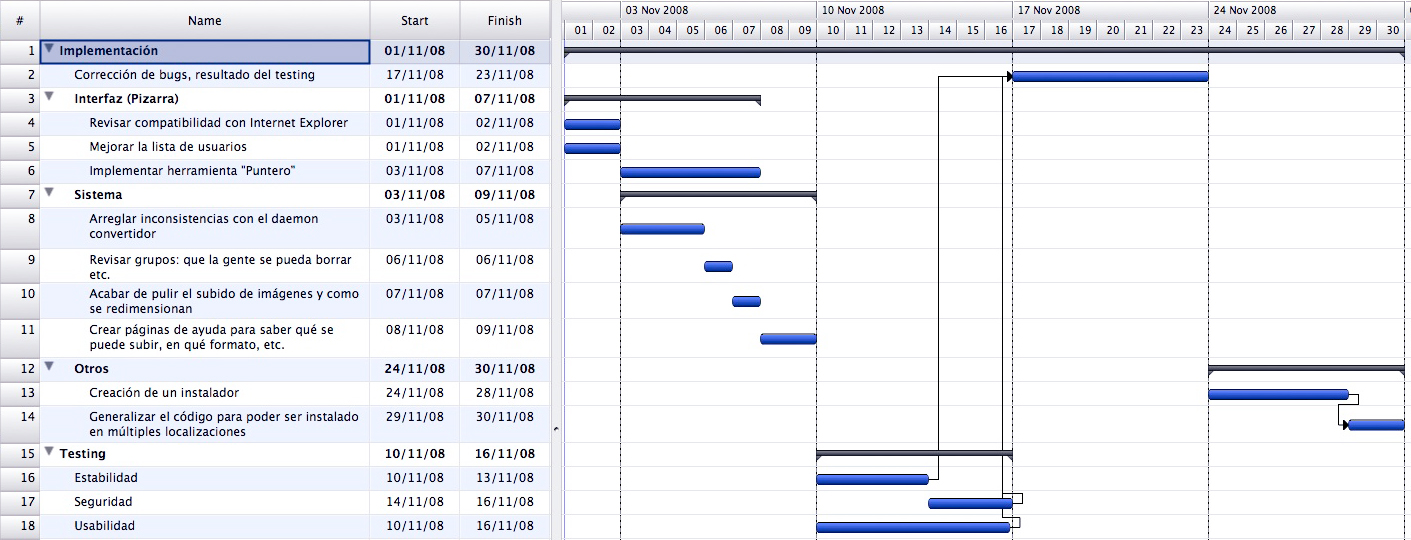
\includegraphics[angle=90,totalheight=1\textheight]{ganttfinal1.jpg}
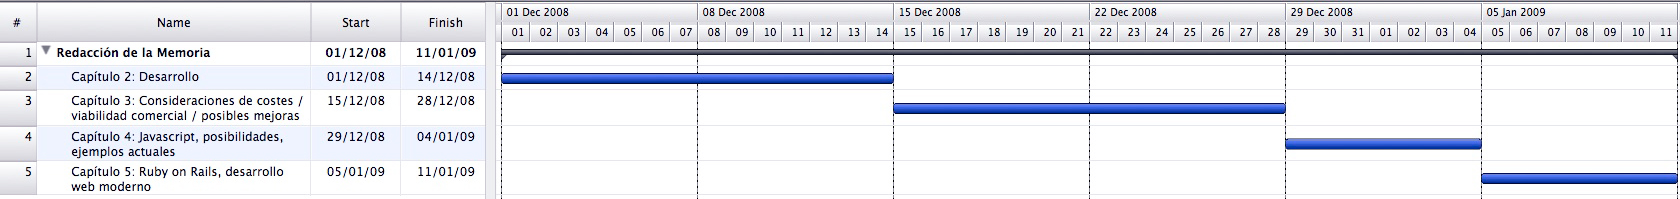
\includegraphics[angle=90,totalheight=1\textheight]{ganttfinal2.jpg}
\end{figure}

\begin{figure}[ht]
\centering
\end{figure}

\end{document}
